\documentclass[12pt]{scrartcl}

\usepackage[utf8]{inputenc}
\usepackage[naustrian]{babel}
\usepackage{caption}
\usepackage{graphicx}
\usepackage{verbatim}
\usepackage[T1]{fontenc}
\usepackage{lmodern}
\usepackage{subcaption}
\usepackage{amsmath}
\usepackage{mathtools}
\usepackage{amsfonts} 
\usepackage{algorithm2e}
\usepackage{listings}
\usepackage{csquotes}

%pdfs
\usepackage{pdfpages}
\usepackage{tikz}

%page borders
\usepackage{geometry}
\geometry{left=2.5cm,right=2.5cm,top=3cm,bottom=2.5cm}

\usepackage{minted}
\setminted {
	%style=igor, %borland, autumn, vs
	encoding=utf-8,
	autogobble,
	tabsize=4,
	linenos,
	breaklines,
	keywordcase=upper,
	%escapeinside=||
	%bgcolor=bg
	%frame=single
}
% binary tree
\usepackage{tikz-qtree}

\newenvironment{code}{\captionsetup{type=listing}}{}

%title/footer/header values
\usepackage{titling}
\title{DES3UE Übung 1}
\author{Elias Leonhardsberger}
\date{\today{}, Hagenberg}

%footer/header
%\usepackage[automark]{scrpage2}
%\pagestyle{headings}
%\clearscrheadfoot
%\ihead{\thetitle}
%\chead{\theauthor}
%\ohead{\today}
%\cfoot{Seite \pagemark}

\begin{document}
\clearpage
\thispagestyle{empty}
\begin{tikzpicture}[remember picture, overlay]
    \node at (current page.center) {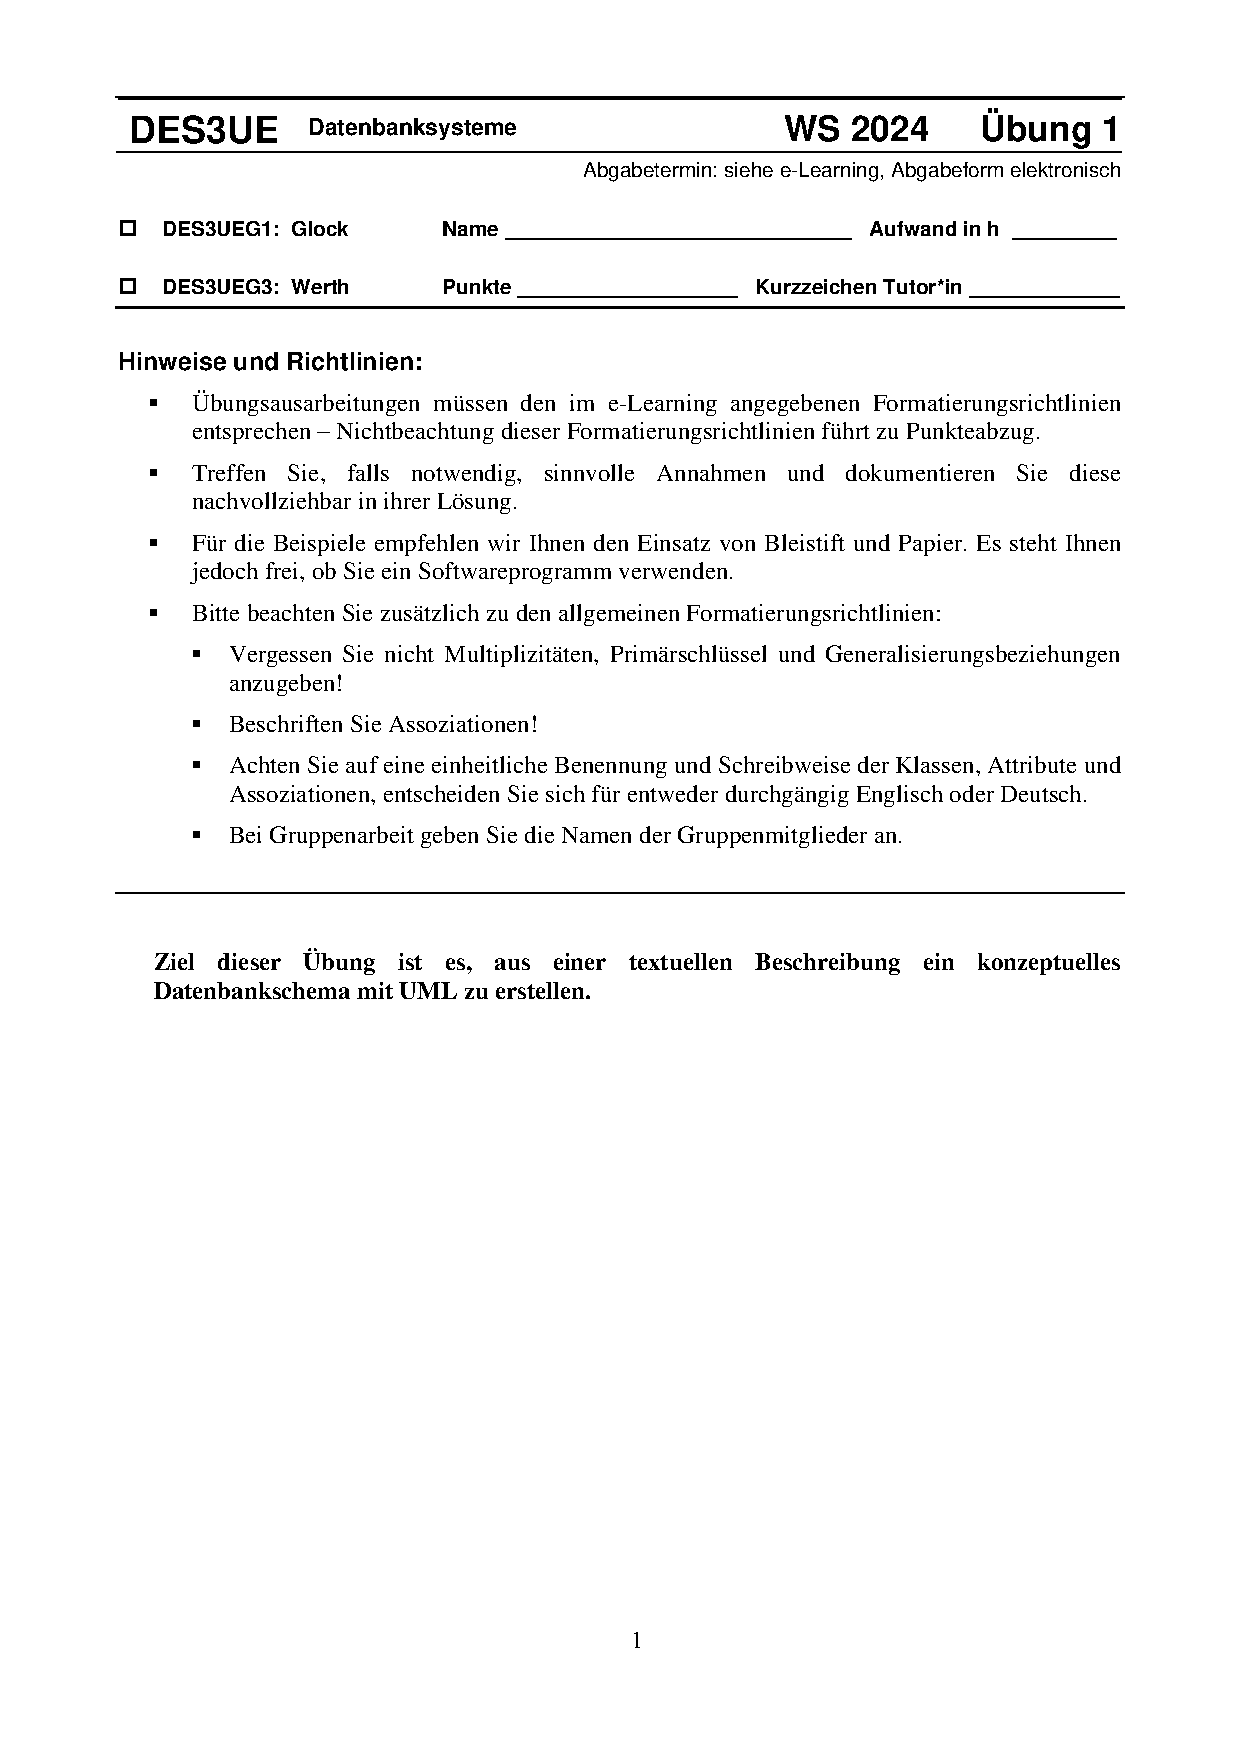
\includegraphics[page=1]{Angabe.pdf}};
    \begin{scope}[shift={(current page.south west)},every node/.style={anchor=base west}]
        \node at (8.5cm, 25.8cm) {\theauthor};
        \node at (17.2cm, 25.8cm) {5};
        \node at (1.87cm, 25.7cm) {X};
    \end{scope}
\end{tikzpicture}

\includepdf[pages=2-5]{Angabe.pdf}

\maketitle
\tableofcontents

\pagebreak

\section{UML Korrekturen}
\subsection{Bestellungen}
\begin{figure}[ht]
    \centering
    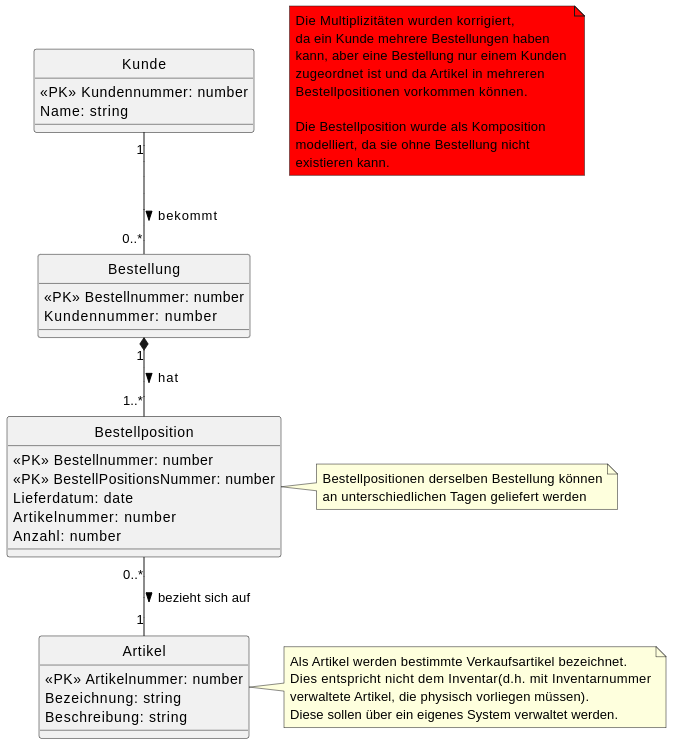
\includegraphics[width=0.9\linewidth]{../UE1_1_1.png}
    \caption{Verbessertes UML Diagram der Aufgabe 1.1 mit Begründungen}
\end{figure}
\pagebreak
\subsection{Rezeptverwaltung}
\begin{figure}[ht]
    \centering
    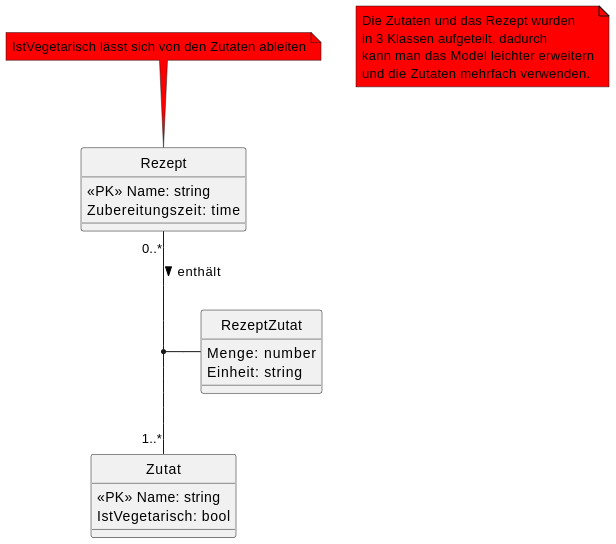
\includegraphics[width=0.9\linewidth]{../UE1_1_2.png}
    \caption{Verbessertes UML Diagram der Aufgabe 1.2 mit Begründungen}
\end{figure}
\pagebreak
\subsection{Anstellungsverhältnisse}
\begin{figure}[ht]
    \centering
    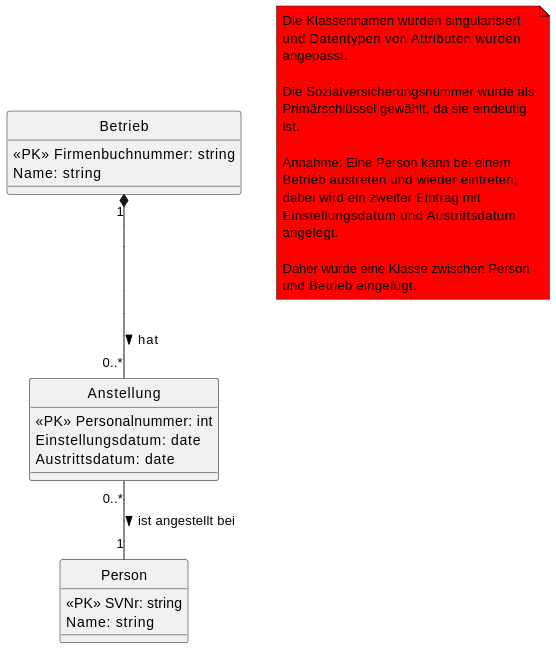
\includegraphics[width=0.9\linewidth]{../UE1_1_3.png}
    \caption{Verbessertes UML Diagram der Aufgabe 1.3 mit Begründungen}
\end{figure}
\pagebreak
\subsection{Studierende}
\begin{figure}[ht]
    \centering
    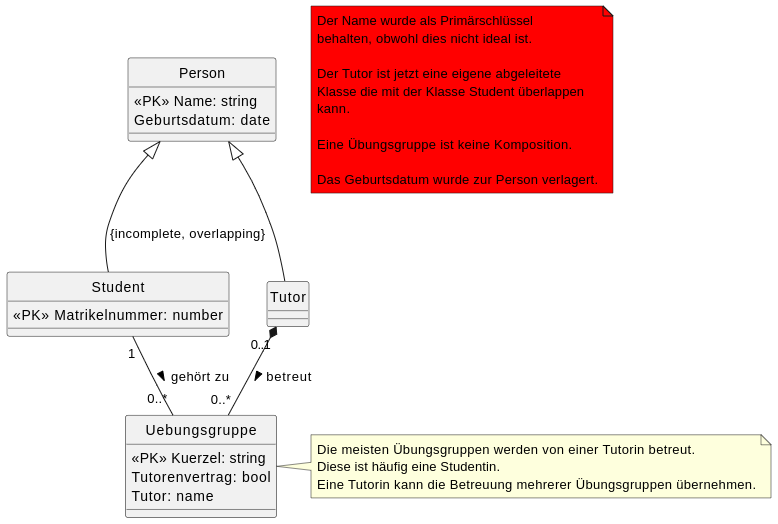
\includegraphics[width=0.9\linewidth]{../UE1_1_4.png}
    \caption{Verbessertes UML Diagram der Aufgabe 1.4 mit Begründungen}
\end{figure}
\pagebreak

\section{Studentisches Hilfssystem}
\subsection{Klassendiagramm}

\begin{figure}[ht]
    \centering
    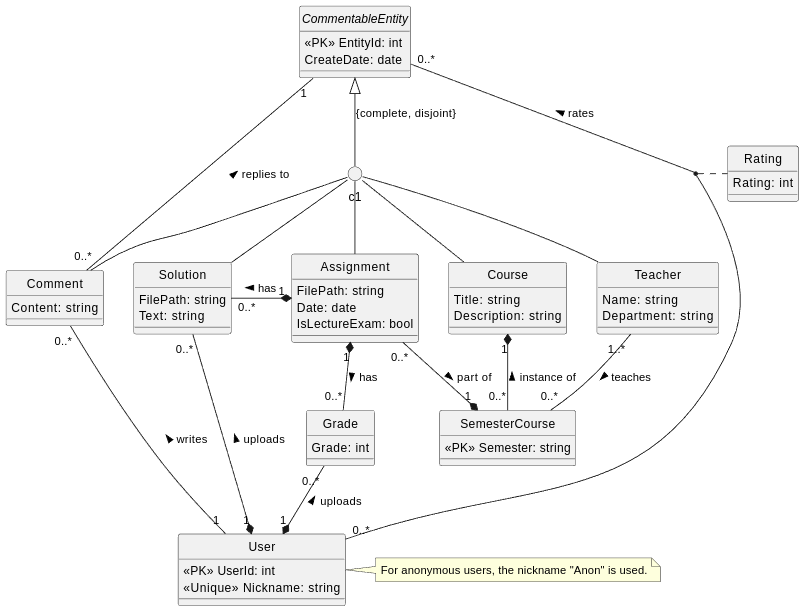
\includegraphics[width=0.9\linewidth]{../UE1_2.png}
    \caption{Klassendiagramm der Aufgabe 2}
\end{figure}

Das Basisdiagram wurde ein wenig angepasst, da \emph{Comments} bereicht kommentierbar sind,
müsste es keine selbstreferenzierende Relation von \emph{Comments} geben.\par

\emph{Grades} und \emph{Solutions} sind keine Beziehungsentitäten,
da \emph{User} mehrere \emph{Grades} und \emph{Solutions} pro \emph{Assingment} hochladen können,
dies ist vor allem für den \enquote{Anon} \emph{User} relevant.\par

Ein Kreis \emph{c1} wurde verwendet um die Vererbung mit PlantUML schöner darzustellen.\par

Da die Sprache im Basisdiagram gemischt war, wurde englisch als Sprache festgelegt entschieden.
\pagebreak

\subsection{SQL-Statements}
\inputminted{sql}{../UE1_2.sql}
\pagebreak

\section{Mensa-Datenbankmodell}
\begin{figure}
    \centering
    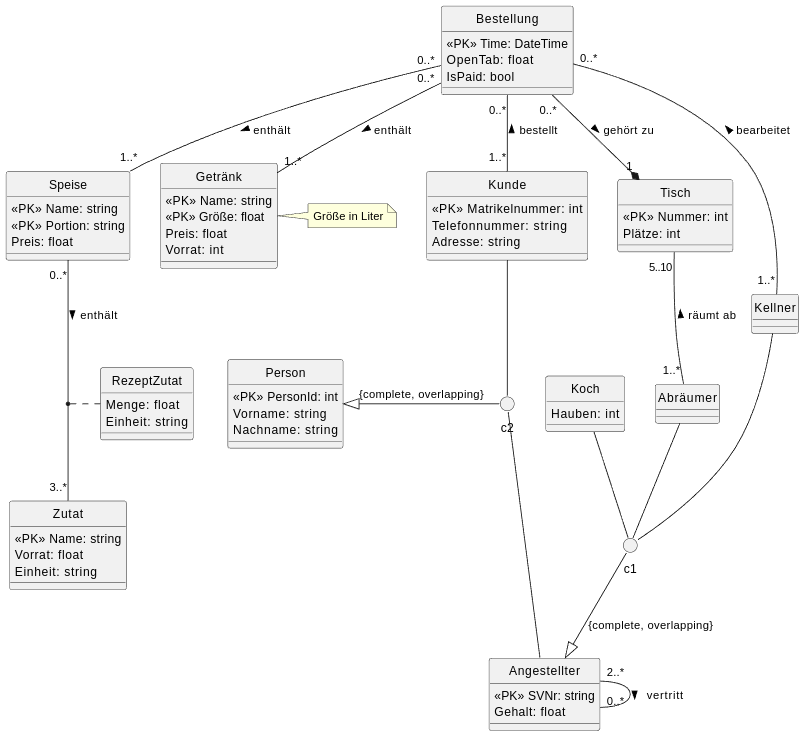
\includegraphics[width=0.9\linewidth]{../UE1_3.png}
    \caption{Klassendiagramm der Aufgabe 3}
\end{figure}

Es wurde angenommen, dass ein \emph{Angestellter} auch als \emph{Kunde} in der Mensa essen kann und,
dass ein \emph{Angestellter} mehrere Rollen(\emph{Koch}, \emph{Kellner}, \emph{Abräumer}) haben kann.
\end{document}